\documentclass{article}
\usepackage[utf8]{inputenc}
\usepackage{tikz}
\usetikzlibrary{positioning}
\usetikzlibrary{shapes}

\begin{document}

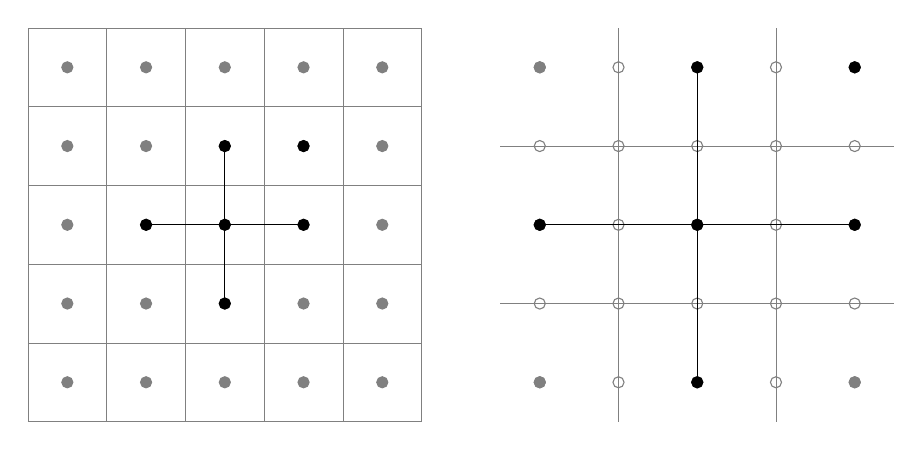
\begin{tikzpicture}
%topleft grid
\draw[step=1cm,gray,very thin] (0,0) grid (5,5);
%topright grid
%\draw[step=1cm,gray,very thin, dashed] (6,0) grid (11,5);
\foreach \x in {7.5,9.5}
{
	\draw[gray, very thin] (\x, 0) -- (\x,5);
}
\foreach \y in {1.5, 3.5}
{
	\draw[gray, very thin] (6, \y) -- (11,\y);
}

%nodes topleft
\foreach \x in {0.5,1.5,2.5,3.5,4.5}
\foreach \y in {0.5,1.5,2.5,3.5,4.5}
{
	\filldraw [gray] (\x,\y) circle (2pt);
}
%left stencil
\filldraw [black] (2.5,1.5) circle (2pt);
\filldraw [black] (2.5,2.5) circle (2pt);
\filldraw [black] (2.5,3.5) circle (2pt);
\filldraw [black] (1.5,2.5) circle (2pt);
\filldraw [black] (3.5,2.5) circle (2pt);
\filldraw [black] (3.5,3.5) circle (2pt);
\draw [black] (1.5, 2.5) -- (3.5,2.5);
\draw [black] (2.5, 1.5) -- (2.5,3.5);

%nodes right
\foreach \x in {0.5,1.5,2.5,3.5,4.5}
\foreach \y in {0.5,1.5,2.5,3.5,4.5}
{
	\draw [gray] (\x+6,\y) circle (2pt);
}
\foreach \x in {0.5,2.5,4.5}
\foreach \y in {0.5,2.5,4.5}
{
	\filldraw [gray] (\x+6,\y) circle (2pt);
}
%right stencil
\filldraw [black] (8.5,0.5) circle (2pt);
\filldraw [black] (8.5,2.5) circle (2pt);
\filldraw [black] (8.5,4.5) circle (2pt);
\filldraw [black] (6.5,2.5) circle (2pt);
\filldraw [black] (10.5,2.5) circle (2pt);
\filldraw [black] (10.5,4.5) circle (2pt);
\draw [black] (6.5, 2.5) -- (10.5,2.5);
\draw [black] (8.5, 0.5) -- (8.5,4.5);
\end{tikzpicture}
\end{document}
